
\begin{figure}[htbp]
    \centering
    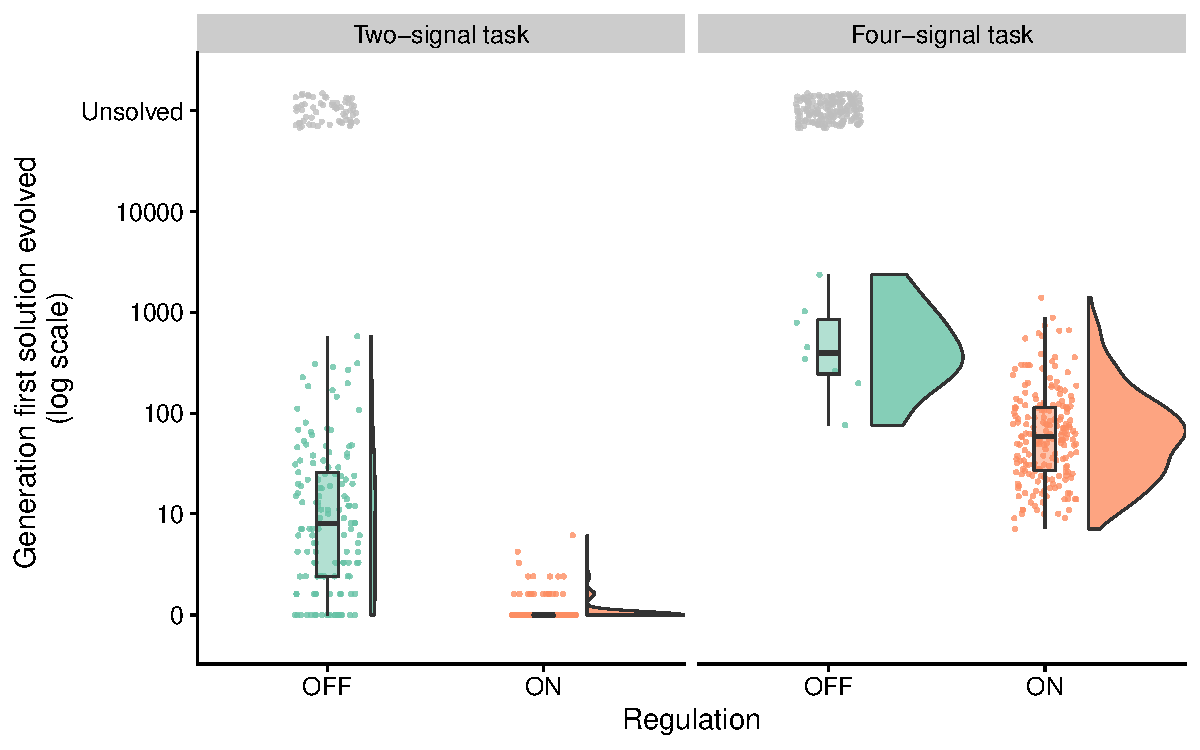
\includegraphics[width=0.7\textwidth]{chapters/05-tag-based-genetic-regulation/media/signal-counting-solve-time-cloud.pdf}
    \caption{\small
    \textbf{Generation at which first solution evolved (log scale) in each successful replicate for the signal-counting problem (raincloud plot \citep{allen_raincloud_2019}).}
    We show data from only those problem difficulties in which solutions evolved (two- and four-signal problems).
    Gray points indicate the number of unsuccessful replicates for each condition.
    For both problem difficulties, regulation-on solutions typically required fewer generations than regulation-off solutions to arise (Wilcoxon rank sum test; two-signal: $p < 10^{-15}$, four-signal: $p < 9\times10^{-05}$). 
    }
    \label{chapter:tag-based-regulation:fig:signal-counting-solve-time}
\end{figure}

% two-signal - p-value < 2.2e-16
% four-signal 8.603e-05